\section{Introduction}\label{sec:intro}

The Software-Defined Networking (SDN) paradigm has brought programmability to the once rigid network ecosystem.
By allowing both control and data planes to evolve independently, SDN has opened new research avenues in networking, including data plane programming.
Notably, the P4 language is a result of the SDN convergence~\cite{Bosshart:14}.
P4 leverages OpenFlow by allowing network admins to program their network in a custom fashion.
Thanks to P4 and recent programmable dataplanes~\cite{Bosshart:13}, network admins can now deploy custom protocols by simply reprogramming the network switches according to their evolving needs, without the need to deploy expensive new hardware. 

\begin{figure}[]
	\centering
	%\begin{tikzpicture}[node distance = 0.5cm, every node/.style={draw}, node font={\footnotesize}]
%%software
%\begin{scope}[every node/.style={draw, chamfered rectangle, chamfered rectangle corners=north east}]
%	\node (globp4) {P4};
%	\node[rectangle, right=of globp4] (compiler) {HDP compiler};
%	\node[below= 0.5cm of compiler] (p4cpu2) { P4};
%	\node[left= of p4cpu2] (p4cpu1) {P4};
%	\node[left= of p4cpu1] (p4fpga1) {P4};
%	\node[right= of p4cpu2] (p4fpga2) {P4};
%	\node[right= of p4fpga2] (p4asic) { P4};
%%%path for the corner of p4 codes
%	\path[draw]  (globp4.before north east) -| (globp4.after north east)
%							  (p4cpu2.before north east) -| (p4cpu2.after north east)
%							  (p4cpu1.before north east) -| (p4cpu1.after north east)
%						      (p4fpga1.before north east) -| (p4fpga1.after north east)
%							  (p4fpga2.before north east) -| (p4fpga2.after north east)
%							  (p4asic.before north east) -| (p4asic.after north east);
%
%%%compilation
%	\begin{scope}[every node/.style={rectangle, draw, align=center}, node distance=0.25cm]
%		\node[below= of p4cpu2] (compcpu2) { CPU\\ comp};
%		\node[below= of p4cpu1] (compcpu1) { CPU\\ comp};
%		\node[below= of p4fpga1] (compfpga1) { FPGA\\ comp};
%		\node[below= of p4fpga2] (compfpga2) { FPGA\\ comp};
%		\node[below= of p4asic] (compasic) { ASIC\\ comp};
%	\end{scope}
%%%processus
%	\begin{scope}[every edge/.style={-Stealth, draw}]
%   \coordinate (midBelowComp) at ($(compiler.south) - (0,0.25)$);
%	\path[draw] (globp4) edge (compiler)
%	    							  (compiler.south) edge (p4cpu2)
%								  ($(compiler.south) - (0.2,0)$) |- ( p4cpu1.north |- midBelowComp) edge (p4cpu1)
%                                  ($(compiler.south) - (0.4,0)$) |- ($( p4fpga1.north |- midBelowComp) + (0,0.1)$) edge (p4fpga1)
%								 ($(compiler.south) + (0.2,0)$) |- ( p4fpga2.north |- midBelowComp) edge (p4fpga2)
%                                  ($(compiler.south) + (0.4,0)$) |- ($( p4asic.north |- midBelowComp) + (0,0.1)$) edge (p4asic)
%								 (p4cpu1) edge (compcpu1)
%								 (p4cpu2) edge (compcpu2)
%								 (p4fpga1) edge (compfpga1)
%								 (p4fpga2) edge (compfpga2)
%								 (p4asic) edge (compasic)
%									;
%	\end{scope}
%
%\end{scope}
%\coordinate (midCPU) at ($(p4cpu1.east |- compcpu1.south) + (0.25cm, -0.5cm)$);
%%%hardware
%\begin{scope}[every node/.style={draw},]
%	\node[left=0.25cm of midCPU, anchor=north east] (cpu1) {CPU\textsubscript{1}};
%	\node[right=0.25cm of midCPU, anchor=north west] (cpu2) {CPU\textsubscript{2}};
%	\node[below=of cpu1, fill=black!20] (fpga1) {FPGA\textsubscript{1}};
%	\node[below=of cpu2] (fpga2) {FPGA\textsubscript{2}};
%	\node[fill=black!20, minimum width=2.25cm, anchor = north] (asic) at ($(midCPU|-fpga2.south) - (0,0.5)$) {ASIC};
%	\node[draw=none,left =0.55 of asic, align=left] (data_label) {};
%	
%\end{scope}
%\node[fit=(cpu1) (cpu2) (fpga1) (fpga2) (asic) (data_label), rounded corners] (platform) {};
%\node[draw=none, anchor=west] at (platform.west |- asic.east) {HDP};
%\node[cloud, draw, aspect=2, inner sep=-2pt, below=0.4cm of asic] (network) {Network};
%\begin{scope}[every edge/.style={Stealth-Stealth, draw}]
%\path (cpu1) edge (cpu2)
%			(cpu1) edge (fpga1)
%			(cpu2) edge (fpga2)
%			(fpga1.south) edge (fpga1.south |- asic.north)
%			(fpga2.south) edge (fpga2.south |- asic.north)
%			;
%\end{scope}
%\begin{scope}[every edge/.style={thick, -Latex, dashed, draw}, every path/.style={thick, dashed}]
%		\path[draw] ($(platform.west |- compfpga1.south) - (0.1,0)$) -- ($(platform.west |- fpga1) - (0.1,0)$)  edge (fpga1)
%								(compfpga2) -- (compfpga2 |- fpga2) edge (fpga2)
%								(compasic) -- (compasic |- asic) edge (asic)
%								(compcpu2) edge (compcpu2.south |- cpu2.north) 
%								(compcpu1) edge (compcpu1.south |- cpu1.north) 
%								;
%	\end{scope}
%\path[Stealth-Stealth, draw] (network) edge (asic.south)
% 							   (network) edge ($(asic.south) + (0.2,0cm)$)
% 							   (network) edge ($(asic.south) - (0.2,0cm)$)
% 							   (network) edge ($(asic.south) + (0.4,0cm)$)
% 							   (network) edge ($(asic.south) - (0.4,0cm)$);
%	\node[draw, anchor = west, fill=black!20](control) at (network.east -| platform.east) { Control-plane};	
%	  \path[densely dashed, Stealth-Stealth, draw] (control) -| ($(platform.south east) - (0.5cm,0)$);
%	\node[fit = (compfpga1) (compasic) (compiler), draw, dash dot dot, thick] (comp) {};
%	\node[draw=none, below left=0 and 0 of comp.north east, align=left] { Compilation\\ Process};
%	\end{tikzpicture}
%	
%	

\tikzset{%
  block/.style    = {draw, very thick, rectangle, minimum height = 2em,
    minimum width = 3em},
  sum/.style      = {draw, circle, node distance = 2cm}, % Adder
  input/.style    = {coordinate}, % Input
  output/.style   = {coordinate} % Output
}
% Defining string as labels of certain blocks.
%\newcommand{\suma}{\Large$+$}
%\newcommand{\inte}{$\displaystyle \int$}
%\newcommand{\derv}{\huge$\frac{d}{dt}$}

\tikzstyle{block} = [draw, rectangle, 
    minimum height=1em, minimum width=3em]
\tikzstyle{sum} = [draw, circle, node distance=1cm]
\tikzstyle{input} = [coordinate]
\tikzstyle{output} = [coordinate]
\tikzstyle{pinstyle} = [pin edge={to-,thin,black}]

\begin{tikzpicture}[auto, node distance=1cm,>=latex']
    \node [input, name=input] {};


    \node [block, below of=input, node distance=.85cm] (cpu) {\small\textbf{PDD\textsubscript{N}}};

    \node [block, right=2 cm of cpu, node distance=.85cm] (cpu1) {\small\textbf{PDD\textsubscript{N}}};
    
\draw[dotted, semithick, name=mm] ($(cpu.north west)+(-2.5cm,+.2cm)$) -- ($(cpu1.north east)+(1cm,+.2cm)$);

    \node [draw=none] at ($(cpu.north west)+(-1.5cm,+.55cm)$) (main) {\scriptsize{\textit{Main Memory}}};


\draw[dotted, semithick] ($(cpu.south west)+(-2.5cm,-.2cm)$) -- ($(cpu1.south east)+(1cm,-.2cm)$);

    \node [draw=none] at ($(cpu.west)+(-1.5cm,-.0cm)$) (hdp) {\scriptsize{\textit{Cache Level N}}};

    \node [block, below of=cpu, node distance=1.75cm] (fpga) {\small\textbf{PDD\textsubscript{2}}};

    \node [draw=none] at ($(fpga.north)+(.0cm,.75cm)$) (dotspdd) {\textbf{$\vdots$}};

    \node [draw=none] at ($(dotspdd)+(1.5cm,-.1cm)$) (dots) {\textbf{$\dots$}};

    \node [draw=none] at ($(dots)+(0cm,.75cm)$) (dotp) {\textbf{$\dots$}};

    \node [draw=none] at ($(dots)+(0cm,-.75cm)$) (dotm) {\textbf{$\dots$}};

    \node [draw=none] at ($(dotm)+(0cm,-1.0cm)$) (dotmm) {\textbf{$\dots$}};


    \node [block, below of=cpu1, node distance=1.75cm] (fpga1) {\small\textbf{PDD\textsubscript{2}}};

    \node [draw=none] at ($(fpga1.north)+(.0cm,.75cm)$) (dotspdd1) {\textbf{$\vdots$}};


\draw[dotted, semithick] ($(fpga.north west)+(-2.5cm,+.2cm)$) -- ($(fpga1.north east)+(1cm,+.2cm)$);

\draw[dotted, semithick] ($(fpga.south west)+(-2.5cm,-.2cm)$) -- ($(fpga1.south east)+(1cm,-.2cm)$);


    \node [draw=none] at ($(fpga.west)+(-1.5cm,-.0cm)$) (ll) {\scriptsize{\textit{Cache Level 2}}};

    \node [draw=none] at ($(ll.north)+(.0cm,.75cm)$) (dotscl) {\textbf{$\vdots$}};

    \node [block, below of=fpga, node distance=1.0cm] (asic) {\small\textbf{PDD\textsubscript{1}}};

    \node [block, below of=fpga1, node distance=1.0cm] (asic1) {\small\textbf{PDD\textsubscript{1}}};



    \node [draw=none] at ($(asic.west)+(-1.5cm,-.0cm)$) (hdp) {\scriptsize{\textit{Cache Level 1}}};

    \node [block,node distance=.85cm, minimum width=7em]  at ($(cpu.north)+(1.5cm,.70cm)$) (controller) {\textbf{Controller}};


	\node[cloud, draw, aspect=2, inner sep=-2pt,minimum width=5em, minimum height=3em] at ($(asic.south)+(1.5cm,-.75cm)$) (network) {\textbf{Network}};

    \node [output, below of=network] (output) {};

    % Once the nodes are placed, connecting them is easy. 
    %%%\draw [thick,<->] (fpga) -- node {} (cpu);
    %%%\draw [thick,<->] (fpga1) -- node {} (cpu1);

    \draw [thick,<->] (cpu) -- node {} ($(dotspdd.center)+(0.0cm,.10cm)$);
    \draw [thick,<->] (fpga) -- node {} ($(dotspdd.south)+(0.0cm,.09cm)$);

    \draw [thick,<->] (cpu1) -- node {} ($(dotspdd1.center)+(0.0cm,.10cm)$);
    \draw [thick,<->] (fpga1) -- node {} ($(dotspdd1.south)+(0.0cm,.09cm)$);
    
    \draw [dashed, <->] (fpga.west) --+(-0.25cm,0) |- node {} (asic);
    \draw [dashed, <->] (cpu.west) --+(-0.25cm,0) |- node {} (fpga);
    \draw [thick,<->] (fpga) -- node {} (asic);
    \draw [very thick,<->] (asic) |- node {} (network);

    \draw [dashed, <->] (fpga1.east) --+(0.25cm,0) |- node {} (asic1);
    \draw [dashed, <->] (cpu1.east) --+(0.25cm,0) |- node {} (fpga1);
    \draw [thick,<->] (fpga1) -- node {} (asic1);
    \draw [very thick,<->] (asic1) |- node {} (network);

    \draw [dashed, <->] (cpu.west)  --+(-0.25cm,0) |- node {} (controller.west);
    \draw [dashed, <->] (cpu1.east) --+(0.25cm,0) |- node {}(controller.east);


    \draw []($(cpu1.north)+(-.65cm,.15cm)$) rectangle ($(asic1.south)+(0.9cm,-.30cm)$);
    
    \draw []($(cpu.north)+(-0.9cm,.15cm)$) rectangle ($(asic.south)+(0.65cm,-.30cm)$);
    
    \node [draw=none] at ($(asic.south west)+(-.075cm,-.15cm)$) (hdp) {\footnotesize{HDP\textsubscript{1}}};
    \node [draw=none] at ($(asic1.south east)+(.075cm,-.15cm)$) (hdp) {\footnotesize{HDP\textsubscript{N}}};

\end{tikzpicture}

	\caption{Reference caching system}
	\label{fig:high_level_network}
\end{figure}

\begin{figure*}[]
	\centering
	\subfloat[Heavy hitter flows]{
	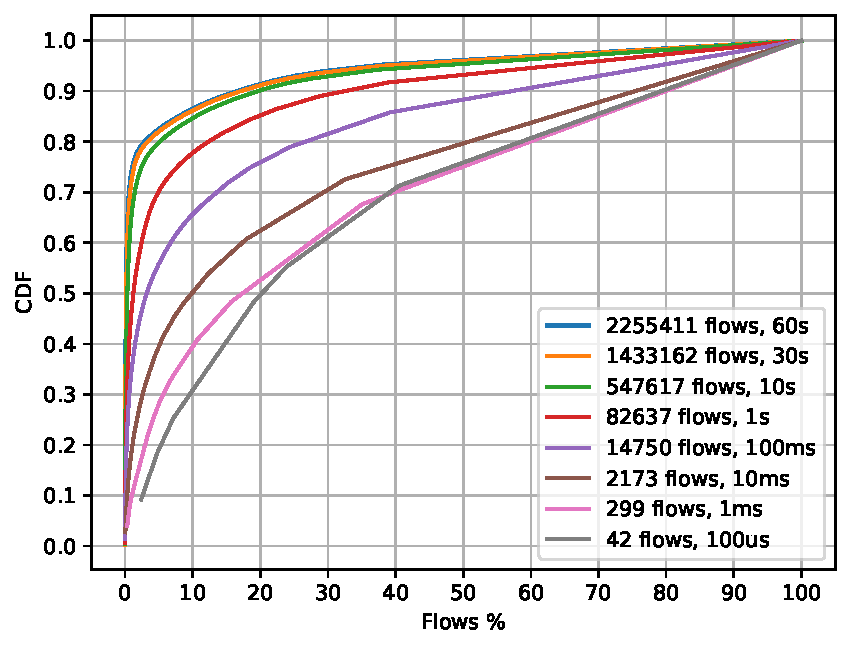
\includegraphics[width=0.25\textwidth]{fig_cdf_pkt.pdf}
	\label{fig:cdf_pkt}
	}
	\subfloat[Size-weighted heavy hitter flows]{
		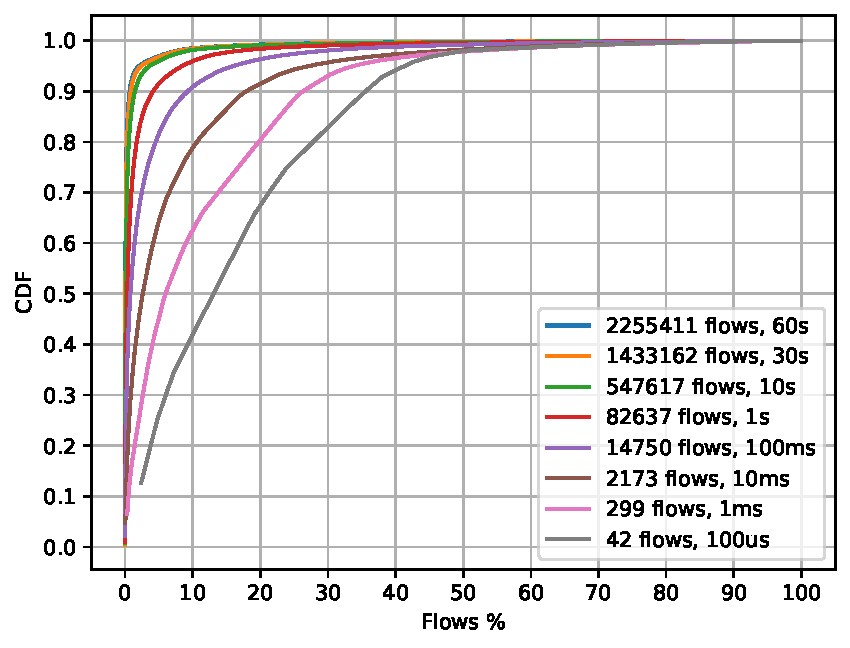
\includegraphics[width=0.25\textwidth]{fig_cdf.pdf}
		\label{fig:cdf}
	}
	\subfloat[Flow duration]{
		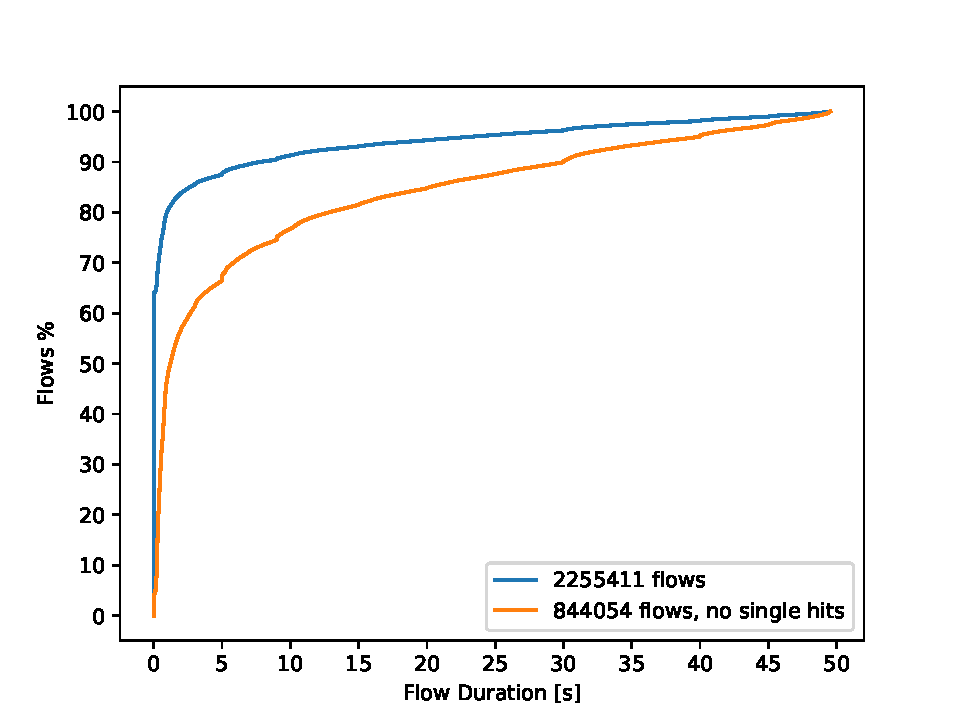
\includegraphics[width=0.25\textwidth]{fig_duration.pdf}
		\label{fig:flow_duration}
	}
	\subfloat[Average flow size]{
		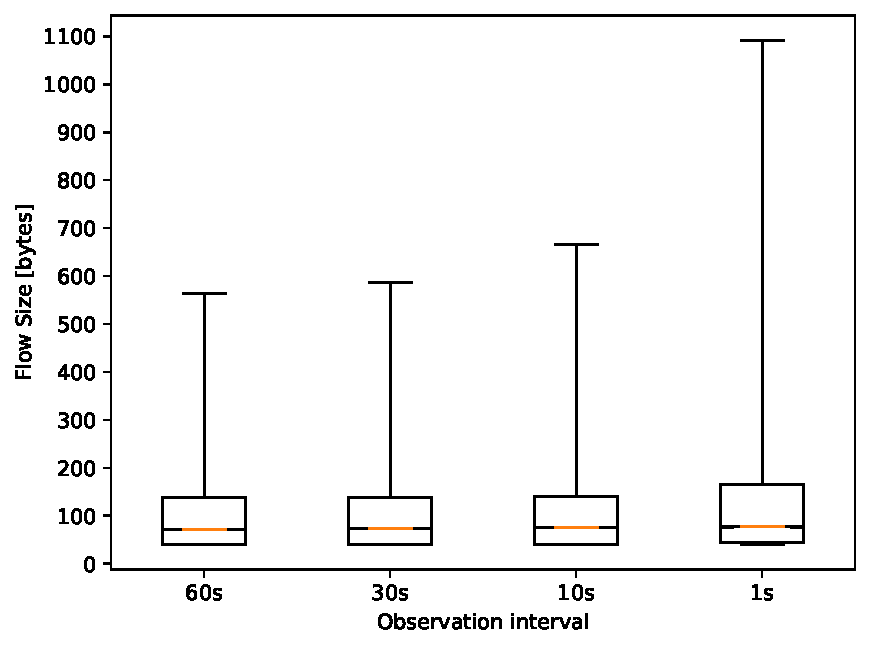
\includegraphics[width=0.25\textwidth]{fig_avg_flow_size.pdf}
		\label{fig:flow_size}
	}
	\caption{CAIDA trace summary}
	\label{fig:traces}
\end{figure*}


However, current requirements of data center networks are such that even state-of-the-art programmable ASICs switches cannot solely meet them.
For instance, 5G mobile communication requires multi-million active sessions ($>$\SI{5}{\mega\nothing}) at terabit rates, stringently low end-to-end latency ($<$\SI{1}{\milli\second}), and likely, new P4-defined custom protocols.

We recently suggested using heterogeneous programmable dataplanes (HDPs) to alleviate data center network switch bottlenecks~\cite{p4eu:18}.
Indeed, using complementary and distinct packet forwarding devices increases the overall switch processing capabilities.
However, research regarding HDPs is still in its infancy with many open questions, such as heterogeneous compilers, the issue of mismatched processing capabilities among devices, and distributed match-tables management.

In this work, we address the issue of distributed match-action table management in HDPs comprising two or more programmable dataplane devices (PDDs), as illustrated in Figure~\ref{fig:high_level_network}.
As an example, an HDP could be made of a programmable ASIC for $PDD_1$, an  FPGA for $PDD_2$, and, a local CPU for $PDD_3$.


To that end, we borrow from the cache hierarchy concept of regular computer systems.
%In our system, a first-level cache is a high-performance but memory limited programmable ASIC.
%The FPGA plays the role of second-level cache, and finally the CPU is the last-level cache.
In our proposed caching system, a first-level cache is a high-performance but memory-limited PDD.
At every cache level, the performance metric $P_{k}$ (throughput in our case) is decreased, in a way where $P_{k-1} >> P_{k} >> P_{k+1}$.
Memory capacity is augmented to $M_{k}$, where $M_{k-1} << M_{k} << M_{k+1}$. 
The performance ratio between two successive cache levels is characterized by a processing slowdown factor $SF$ defined as $SF_{k} = \left(\frac{P_{k}}{P_{k-1}}\right)^{-1}$.


However, match-action caching is fairly different from CPU caches.
First, temporal and spatial data locality is less predictable in network systems.
Second, memory is scarce and the processing flexibility is limited in network switches, thus, complex cache policies may not be suitable.
Third, due to dynamic traffic changes, a cache system needs to rapidly adapt to diversified workloads.
As a consequence, traditional computer caching schemes cannot be directly applied in heterogeneous match table caching systems. 

%Thus, we propose a match-action cache policer split into the forwarding devices.
%We use online traffic hitters to estimate which match-action entries are candidates to be promoted/evicted to/from another cache level.
%We are inspired in previous works on flow caching \cite{casado:2008,Katta:2014,Pfaff:15} and on heuristic dataplane-based traffic hitters \cite{Sivaraman:17} aiming to maintain line-rate throughput and required cache update rate while minimizing the usage of scarce memory resources available in each device and reducing processing latency.

To properly characterize the aforementioned issues, we evaluated the feasibility of such an HDP caching system by characterizing an up-to-date data center network traffic to understand its temporal locality.
Following the traffic analysis, we conducted cache simulations to choose realistic cache policies to be implemented in HDPs.
Finally, we evaluated which cache policies are optimized for current programmable dataplanes and how they can be described in P4.

To the best of our knowledge, this work is the first to consider match-action table management for HDPs.
The contributions of this work are as follows: 

\begin{itemize}[noitemsep,topsep=0pt]
	\item an open-source match-action cache policer for HDPs;
	\item a real-world network traffic analysis to derive match-action caching premises~(\S\ref{sec:traffic});
	\item an evaluation of cache policies in the context of programmable dataplanes~(\S\ref{sec:policies}); and
	\item a model to estimate the performance and overhead of a match-action caching system in an HDP~(\S\ref{sec:cache_results}).
\end{itemize}
